\documentclass{../exhibit}

\title{Pirate Chains}

%% Font
\usepackage{imfellEnglish}
\usepackage[T1]{fontenc}
\raggedright

\usepackage{background}

\backgroundsetup{
scale=1,
color=black,
opacity=0.4,
angle=0,
contents={%
  \includegraphics[height=\paperheight]{mapBackground.jpg}%%https://upload.wikimedia.org/wikipedia/commons/8/81/Nautical_chart_of_the_West_Indies_1797.jpg
  }%
}




%% For the context
%% https://tex.stackexchange.com/questions/86150/torn-page-effect/86151#86151
\usepackage{tikz}
\usetikzlibrary{decorations.pathmorphing}
\definecolor{paper}{RGB}{239,227,157}





\renewcommand{\maketitle}{ %
  \begin{center}
    \scalebox{8}{\thetitle}
  \end{center}
  
\begin{tabular*}{\textwidth}{c @{\extracolsep{\fill}} c}  
\resizebox{4in}{!}{\begin{minipage}[b]{3in}\huge\directions\end{minipage}} &
  \resizebox{4in}{!}{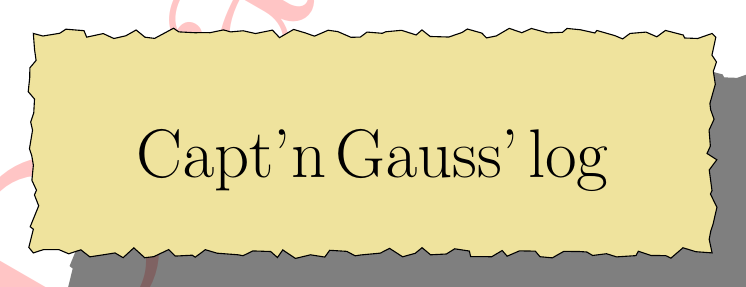
\begin{tikzpicture}[pencildraw/.style={ %
    decorate,
    decoration={random steps,segment length=4pt,amplitude=2pt}
    } %
]
\node[
preaction={fill=black,opacity=.5,transform canvas={xshift=.5cm,yshift=-.5cm}},
pencildraw,draw,fill=paper,text width=3in,inner sep=.5cm] 
{\begin{center}\Huge Capt'n Gauss' log \end{center}\vspace{.7cm} {\huge\context}};
\end{tikzpicture}}

\end{tabular*}

\vfill

\includegraphics[width=3in]{logoPirate.png}\hfill \includegraphics[width=2in]{bammLogo.png}


}


\begin{document}

\begin{context}
  As the sun set on the horizon, I felt a sense of satisfaction wash over me. I may be a math pirate and I enjoy a good bit of arithmetic. I'll be back at it again tomorrow, buildin' me chain of problems ever longer.
\end{context}

\begin{directions}
Take one of the problems written on small pieces of paper.

When you finish a problem, you will add it to a chain of papers by using a stapler.

We will try to make the chain as long as we can!

Each piece of paper will be connected to the next one.
\end{directions}

\begin{example}
\end{example}

\begin{mathConnections}
  https://bartsnapp.github.io/Math-Outreach-Exhibits/arithmeticChain/
\end{mathConnections}
\end{document}
